% Leitende und dielektrische Kugel im homogenen Feld E0 ez (Legendre-Ansatz, l = 1)
% Gemeinsamer Stil für alle Abbildungen (TikZ -> SVG, siehe figures/build.mjs).
%
% Farben sind Platzhalter ("Sentinels"): build.mjs ersetzt sie im SVG durch
% CSS-Variablen, damit die Abbildungen im hellen und dunklen Modus passen.
% Andere Farben (auch schwarz/weiß) bricht der Build mit Fehler ab.
%
%   fg    Linien, Beschriftung          -> --dark
%   mu    Hilfslinien, Achsen, Maße      -> --gray
%   acc   das eine Konzept der Abbildung -> --secondary (Lime/Oliv)
%   blue  zweite Größe, negative Ladung  -> --fig-blue
%   warm  dritte Größe, positive Ladung  -> --fig-warm
%   bg    Seitenhintergrund (Aussparen)  -> --light
%
% Kein \clip verwenden: pdftocairo macht daraus Clip-Gruppen, in denen exakt
% waagerechte/senkrechte Linien verschwinden. Berechnete Kurven schneidet
% gen/*.py selbst am Rahmen ab.
\documentclass[tikz,border=3pt]{standalone}
\usepackage{amsmath,amssymb,bm}
% Text serifenlos wie die Seite, Mathe in Computer Modern wie KaTeX
\renewcommand{\familydefault}{\sfdefault}
\usetikzlibrary{arrows.meta,calc,decorations.markings,patterns,3d,positioning,angles,quotes}

\definecolor{fg}{RGB}{1,2,3}
\definecolor{mu}{RGB}{4,5,6}
\definecolor{acc}{RGB}{7,8,9}
\definecolor{blue}{RGB}{10,11,12}
\definecolor{warm}{RGB}{13,14,15}
\definecolor{bg}{RGB}{16,17,18}

% Vektoren wie auf der Website (KaTeX \mathbf)
\newcommand{\vv}[1]{\mathbf{#1}}

\tikzset{
  every picture/.style={fg, line width=0.8pt, line cap=round, line join=round,
    >={Stealth[length=5.5pt,width=4.4pt]}},
  every node/.style={font=\small},
  % Linientypen
  main/.style={line width=0.9pt},
  thin/.style={line width=0.5pt},
  aux/.style={mu, line width=0.5pt, dash pattern=on 2.5pt off 2pt},
  axis/.style={mu, line width=0.6pt, ->},
  vec/.style={line width=1.1pt, ->},
  field/.style={line width=0.7pt, postaction={decorate},
    decoration={markings, mark=at position #1 with {\arrow{Stealth[length=4.5pt,width=3.6pt]}}}},
  field/.default=0.5,
  % Flächen
  soft/.style={fill=#1, fill opacity=0.14},
  soft/.default=acc,
  % Ladungen
  qpos/.style={circle, fill=warm, inner sep=0pt, minimum size=9pt,
    path picture={\draw[bg, line width=0.9pt] ($(path picture bounding box.center)+(-2pt,0)$) -- +(4pt,0)
      ($(path picture bounding box.center)+(0,-2pt)$) -- +(0,4pt);}},
  qneg/.style={circle, fill=blue, inner sep=0pt, minimum size=9pt,
    path picture={\draw[bg, line width=0.9pt] ($(path picture bounding box.center)+(-2pt,0)$) -- +(4pt,0);}},
  dot/.style={circle, fill=fg, inner sep=0pt, minimum size=3pt},
  % Beschriftung mit Aussparung, damit Linien den Text nicht kreuzen
  lbl/.style={fill=bg, inner sep=1.5pt},
  % Icons: kräftigere Linien, keine Schrift
  icon/.style={line width=1.6pt, >={Stealth[length=6pt,width=5pt]}},
}

\begin{document}
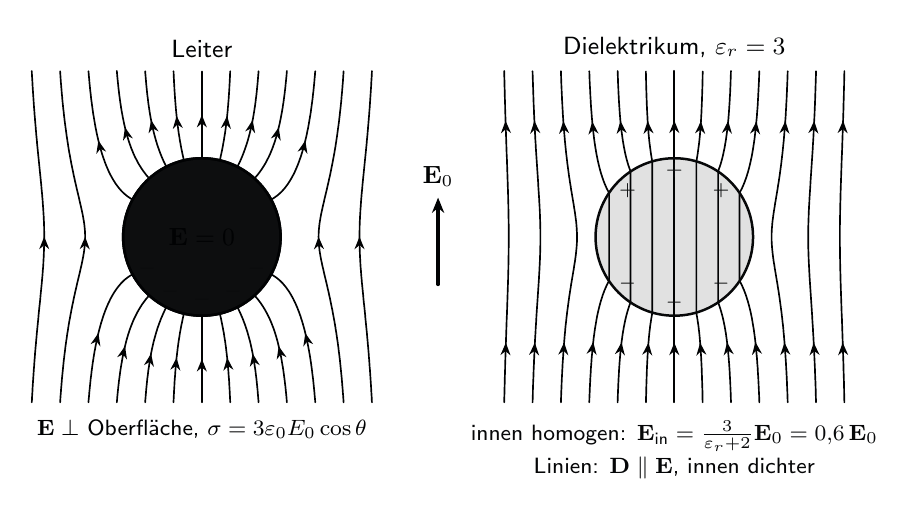
\begin{tikzpicture}
  % ---------- Leiter ----------
  \begin{scope}
    \draw[field=0.5, line width=0.6pt] plot coordinates {(-2.160,-2.100) (-2.158,-2.070) (-2.157,-2.040) (-2.155,-2.010) (-2.153,-1.980) (-2.151,-1.950) (-2.150,-1.920) (-2.148,-1.890) (-2.146,-1.860) (-2.144,-1.830) (-2.142,-1.801) (-2.140,-1.771) (-2.138,-1.741) (-2.136,-1.711) (-2.134,-1.681) (-2.131,-1.651) (-2.129,-1.621) (-2.127,-1.591) (-2.125,-1.561) (-2.122,-1.531) (-2.120,-1.501) (-2.118,-1.471) (-2.115,-1.442) (-2.113,-1.412) (-2.110,-1.382) (-2.107,-1.352) (-2.105,-1.322) (-2.102,-1.292) (-2.099,-1.262) (-2.097,-1.232) (-2.094,-1.202) (-2.091,-1.173) (-2.088,-1.143) (-2.085,-1.113) (-2.082,-1.083) (-2.079,-1.053) (-2.076,-1.023) (-2.074,-0.993) (-2.071,-0.964) (-2.068,-0.934) (-2.065,-0.904) (-2.062,-0.874) (-2.058,-0.844) (-2.055,-0.814) (-2.052,-0.785) (-2.050,-0.755) (-2.047,-0.725) (-2.044,-0.695) (-2.041,-0.665) (-2.038,-0.635) (-2.035,-0.605) (-2.032,-0.576) (-2.030,-0.546) (-2.027,-0.516) (-2.024,-0.486) (-2.022,-0.456) (-2.020,-0.426) (-2.017,-0.396) (-2.015,-0.366) (-2.013,-0.336) (-2.012,-0.306) (-2.010,-0.276) (-2.008,-0.246) (-2.007,-0.216) (-2.006,-0.186) (-2.005,-0.156) (-2.004,-0.127) (-2.003,-0.097) (-2.002,-0.067) (-2.002,-0.037) (-2.002,-0.007) (-2.002,0.023) (-2.002,0.053) (-2.003,0.083) (-2.003,0.113) (-2.004,0.143) (-2.005,0.173) (-2.006,0.203) (-2.008,0.233) (-2.009,0.263) (-2.011,0.293) (-2.013,0.323) (-2.014,0.353) (-2.017,0.383) (-2.019,0.413) (-2.021,0.443) (-2.023,0.473) (-2.026,0.503) (-2.028,0.533) (-2.031,0.563) (-2.034,0.592) (-2.037,0.622) (-2.039,0.652) (-2.042,0.682) (-2.045,0.712) (-2.048,0.742) (-2.051,0.772) (-2.054,0.801) (-2.057,0.831) (-2.060,0.861) (-2.063,0.891) (-2.066,0.921) (-2.069,0.951) (-2.072,0.981) (-2.075,1.010) (-2.078,1.040) (-2.081,1.070) (-2.084,1.100) (-2.087,1.130) (-2.090,1.160) (-2.093,1.190) (-2.095,1.219) (-2.098,1.249) (-2.101,1.279) (-2.104,1.309) (-2.106,1.339) (-2.109,1.369) (-2.111,1.399) (-2.114,1.429) (-2.116,1.458) (-2.119,1.488) (-2.121,1.518) (-2.124,1.548) (-2.126,1.578) (-2.128,1.608) (-2.131,1.638) (-2.133,1.668) (-2.135,1.698) (-2.137,1.728) (-2.139,1.758) (-2.141,1.788) (-2.143,1.817) (-2.145,1.847) (-2.147,1.877) (-2.149,1.907) (-2.151,1.937) (-2.152,1.967) (-2.154,1.997) (-2.156,2.027) (-2.158,2.057) (-2.159,2.087) (-2.160,2.107)};
\draw[field=0.5, line width=0.6pt] plot coordinates {(-1.800,-2.100) (-1.798,-2.070) (-1.796,-2.040) (-1.794,-2.010) (-1.791,-1.980) (-1.789,-1.950) (-1.787,-1.920) (-1.784,-1.891) (-1.782,-1.861) (-1.779,-1.831) (-1.777,-1.801) (-1.774,-1.771) (-1.771,-1.741) (-1.768,-1.711) (-1.765,-1.681) (-1.762,-1.652) (-1.759,-1.622) (-1.756,-1.592) (-1.753,-1.562) (-1.749,-1.532) (-1.746,-1.503) (-1.742,-1.473) (-1.738,-1.443) (-1.735,-1.413) (-1.731,-1.383) (-1.727,-1.354) (-1.723,-1.324) (-1.718,-1.294) (-1.714,-1.265) (-1.710,-1.235) (-1.705,-1.205) (-1.700,-1.176) (-1.696,-1.146) (-1.691,-1.116) (-1.686,-1.087) (-1.681,-1.057) (-1.675,-1.028) (-1.670,-0.998) (-1.664,-0.969) (-1.659,-0.939) (-1.653,-0.910) (-1.647,-0.880) (-1.641,-0.851) (-1.635,-0.822) (-1.629,-0.792) (-1.623,-0.763) (-1.616,-0.734) (-1.610,-0.704) (-1.603,-0.675) (-1.596,-0.646) (-1.590,-0.617) (-1.583,-0.587) (-1.576,-0.558) (-1.569,-0.529) (-1.562,-0.500) (-1.555,-0.471) (-1.548,-0.441) (-1.542,-0.412) (-1.535,-0.383) (-1.528,-0.354) (-1.522,-0.324) (-1.516,-0.295) (-1.510,-0.266) (-1.505,-0.236) (-1.500,-0.206) (-1.495,-0.177) (-1.492,-0.147) (-1.488,-0.117) (-1.486,-0.087) (-1.484,-0.057) (-1.483,-0.027) (-1.482,0.003) (-1.483,0.033) (-1.484,0.063) (-1.486,0.092) (-1.489,0.122) (-1.492,0.152) (-1.496,0.182) (-1.501,0.212) (-1.506,0.241) (-1.511,0.271) (-1.517,0.300) (-1.523,0.329) (-1.530,0.359) (-1.536,0.388) (-1.543,0.417) (-1.550,0.446) (-1.556,0.476) (-1.563,0.505) (-1.570,0.534) (-1.577,0.563) (-1.584,0.592) (-1.591,0.622) (-1.597,0.651) (-1.604,0.680) (-1.611,0.709) (-1.617,0.739) (-1.624,0.768) (-1.630,0.797) (-1.636,0.827) (-1.642,0.856) (-1.648,0.885) (-1.654,0.915) (-1.660,0.944) (-1.665,0.974) (-1.671,1.003) (-1.676,1.033) (-1.682,1.062) (-1.687,1.092) (-1.692,1.122) (-1.697,1.151) (-1.701,1.181) (-1.706,1.210) (-1.710,1.240) (-1.715,1.270) (-1.719,1.299) (-1.723,1.329) (-1.727,1.359) (-1.731,1.389) (-1.735,1.418) (-1.739,1.448) (-1.743,1.478) (-1.746,1.508) (-1.750,1.537) (-1.753,1.567) (-1.756,1.597) (-1.760,1.627) (-1.763,1.657) (-1.766,1.687) (-1.769,1.716) (-1.772,1.746) (-1.774,1.776) (-1.777,1.806) (-1.780,1.836) (-1.782,1.866) (-1.785,1.896) (-1.787,1.926) (-1.790,1.956) (-1.792,1.985) (-1.794,2.015) (-1.796,2.045) (-1.798,2.075) (-1.800,2.105)};
\draw[field=0.5, line width=0.6pt] plot coordinates {(-1.440,-2.100) (-1.438,-2.070) (-1.435,-2.040) (-1.432,-2.010) (-1.430,-1.980) (-1.427,-1.951) (-1.424,-1.921) (-1.421,-1.891) (-1.418,-1.861) (-1.415,-1.831) (-1.412,-1.801) (-1.408,-1.772) (-1.404,-1.742) (-1.401,-1.712) (-1.397,-1.682) (-1.393,-1.653) (-1.389,-1.623) (-1.385,-1.593) (-1.380,-1.563) (-1.376,-1.534) (-1.371,-1.504) (-1.366,-1.475) (-1.361,-1.445) (-1.355,-1.416) (-1.350,-1.386) (-1.344,-1.357) (-1.338,-1.327) (-1.332,-1.298) (-1.325,-1.269) (-1.318,-1.239) (-1.311,-1.210) (-1.304,-1.181) (-1.296,-1.152) (-1.288,-1.123) (-1.280,-1.094) (-1.271,-1.066) (-1.262,-1.037) (-1.253,-1.009) (-1.243,-0.980) (-1.233,-0.952) (-1.222,-0.924) (-1.211,-0.896) (-1.199,-0.868) (-1.187,-0.841) (-1.174,-0.814) (-1.161,-0.787) (-1.147,-0.761) (-1.132,-0.735) (-1.117,-0.709) (-1.100,-0.684) (-1.083,-0.659) (-1.065,-0.635) (-1.046,-0.612) (-1.027,-0.589) (-1.006,-0.568) (-0.984,-0.547) (-0.961,-0.528) (-0.937,-0.510) (-0.912,-0.493) (-0.886,-0.478) (-0.880,-0.474)};
\draw[field=0.5, line width=0.6pt] plot coordinates {(-0.880,0.474) (-0.898,0.485) (-0.923,0.501) (-0.948,0.519) (-0.971,0.537) (-0.993,0.557) (-1.015,0.578) (-1.035,0.600) (-1.055,0.623) (-1.073,0.647) (-1.091,0.671) (-1.107,0.696) (-1.123,0.721) (-1.138,0.747) (-1.153,0.774) (-1.167,0.800) (-1.180,0.827) (-1.192,0.854) (-1.204,0.882) (-1.216,0.910) (-1.227,0.938) (-1.237,0.966) (-1.247,0.994) (-1.257,1.022) (-1.266,1.051) (-1.275,1.080) (-1.283,1.108) (-1.292,1.137) (-1.299,1.166) (-1.307,1.195) (-1.314,1.224) (-1.321,1.254) (-1.328,1.283) (-1.334,1.312) (-1.340,1.342) (-1.346,1.371) (-1.352,1.400) (-1.357,1.430) (-1.362,1.459) (-1.367,1.489) (-1.372,1.519) (-1.377,1.548) (-1.382,1.578) (-1.386,1.608) (-1.390,1.637) (-1.394,1.667) (-1.398,1.697) (-1.402,1.727) (-1.406,1.756) (-1.409,1.786) (-1.412,1.816) (-1.416,1.846) (-1.419,1.876) (-1.422,1.905) (-1.425,1.935) (-1.428,1.965) (-1.430,1.995) (-1.433,2.025) (-1.436,2.055) (-1.438,2.085) (-1.440,2.105)};
\draw[field=0.5, line width=0.6pt] plot coordinates {(-1.080,-2.100) (-1.077,-2.070) (-1.075,-2.040) (-1.072,-2.010) (-1.069,-1.980) (-1.066,-1.951) (-1.063,-1.921) (-1.060,-1.891) (-1.056,-1.861) (-1.053,-1.831) (-1.049,-1.802) (-1.045,-1.772) (-1.041,-1.742) (-1.037,-1.712) (-1.033,-1.683) (-1.028,-1.653) (-1.023,-1.623) (-1.018,-1.594) (-1.013,-1.564) (-1.008,-1.535) (-1.002,-1.505) (-0.996,-1.476) (-0.990,-1.447) (-0.983,-1.417) (-0.976,-1.388) (-0.969,-1.359) (-0.962,-1.330) (-0.954,-1.301) (-0.946,-1.272) (-0.937,-1.243) (-0.928,-1.215) (-0.919,-1.186) (-0.909,-1.158) (-0.898,-1.130) (-0.887,-1.102) (-0.876,-1.074) (-0.864,-1.047) (-0.851,-1.019) (-0.838,-0.993) (-0.824,-0.966) (-0.810,-0.940) (-0.795,-0.914) (-0.779,-0.888) (-0.763,-0.863) (-0.746,-0.838) (-0.728,-0.814) (-0.710,-0.790) (-0.690,-0.767) (-0.671,-0.745) (-0.669,-0.743)};
\draw[field=0.5, line width=0.6pt] plot coordinates {(-0.669,0.743) (-0.682,0.759) (-0.702,0.782) (-0.720,0.805) (-0.738,0.829) (-0.756,0.854) (-0.772,0.879) (-0.788,0.904) (-0.804,0.930) (-0.818,0.956) (-0.832,0.983) (-0.846,1.010) (-0.859,1.037) (-0.871,1.064) (-0.882,1.092) (-0.894,1.120) (-0.904,1.148) (-0.914,1.176) (-0.924,1.204) (-0.933,1.233) (-0.942,1.262) (-0.950,1.290) (-0.958,1.319) (-0.966,1.348) (-0.973,1.378) (-0.980,1.407) (-0.987,1.436) (-0.993,1.465) (-0.999,1.495) (-1.005,1.524) (-1.010,1.554) (-1.016,1.583) (-1.021,1.613) (-1.026,1.642) (-1.030,1.672) (-1.035,1.702) (-1.039,1.731) (-1.043,1.761) (-1.047,1.791) (-1.051,1.821) (-1.054,1.850) (-1.058,1.880) (-1.061,1.910) (-1.064,1.940) (-1.067,1.970) (-1.070,1.999) (-1.073,2.029) (-1.076,2.059) (-1.078,2.089) (-1.080,2.109)};
\draw[field=0.5, line width=0.6pt] plot coordinates {(-0.720,-2.100) (-0.718,-2.070) (-0.715,-2.040) (-0.713,-2.010) (-0.710,-1.980) (-0.708,-1.950) (-0.705,-1.921) (-0.702,-1.891) (-0.699,-1.861) (-0.696,-1.831) (-0.693,-1.801) (-0.689,-1.771) (-0.685,-1.742) (-0.682,-1.712) (-0.678,-1.682) (-0.673,-1.653) (-0.669,-1.623) (-0.664,-1.593) (-0.660,-1.564) (-0.655,-1.534) (-0.649,-1.504) (-0.644,-1.475) (-0.638,-1.446) (-0.632,-1.416) (-0.625,-1.387) (-0.619,-1.358) (-0.612,-1.328) (-0.604,-1.299) (-0.596,-1.270) (-0.588,-1.242) (-0.580,-1.213) (-0.571,-1.184) (-0.562,-1.156) (-0.552,-1.127) (-0.542,-1.099) (-0.531,-1.071) (-0.521,-1.043) (-0.509,-1.015) (-0.497,-0.988) (-0.485,-0.960) (-0.472,-0.933) (-0.459,-0.906) (-0.452,-0.892)};
\draw[field=0.5, line width=0.6pt] plot coordinates {(-0.452,0.892) (-0.461,0.911) (-0.474,0.938) (-0.487,0.965) (-0.499,0.992) (-0.511,1.020) (-0.522,1.048) (-0.533,1.076) (-0.543,1.104) (-0.553,1.132) (-0.563,1.161) (-0.572,1.189) (-0.581,1.218) (-0.589,1.247) (-0.597,1.276) (-0.605,1.305) (-0.612,1.334) (-0.619,1.363) (-0.626,1.392) (-0.632,1.421) (-0.638,1.451) (-0.644,1.480) (-0.650,1.510) (-0.655,1.539) (-0.660,1.569) (-0.665,1.599) (-0.669,1.628) (-0.674,1.658) (-0.678,1.688) (-0.682,1.717) (-0.685,1.747) (-0.689,1.777) (-0.693,1.807) (-0.696,1.836) (-0.699,1.866) (-0.702,1.896) (-0.705,1.926) (-0.708,1.956) (-0.710,1.986) (-0.713,2.016) (-0.715,2.046) (-0.718,2.075) (-0.720,2.105)};
\draw[field=0.5, line width=0.6pt] plot coordinates {(-0.360,-2.100) (-0.359,-2.070) (-0.357,-2.040) (-0.356,-2.010) (-0.354,-1.980) (-0.353,-1.950) (-0.351,-1.920) (-0.349,-1.890) (-0.348,-1.860) (-0.346,-1.830) (-0.344,-1.800) (-0.341,-1.771) (-0.339,-1.741) (-0.337,-1.711) (-0.335,-1.681) (-0.332,-1.651) (-0.329,-1.621) (-0.327,-1.591) (-0.324,-1.561) (-0.321,-1.531) (-0.317,-1.502) (-0.314,-1.472) (-0.310,-1.442) (-0.307,-1.412) (-0.303,-1.383) (-0.299,-1.353) (-0.295,-1.323) (-0.290,-1.293) (-0.285,-1.264) (-0.281,-1.234) (-0.276,-1.205) (-0.270,-1.175) (-0.265,-1.146) (-0.259,-1.116) (-0.253,-1.087) (-0.247,-1.057) (-0.241,-1.028) (-0.234,-0.999) (-0.228,-0.974)};
\draw[field=0.5, line width=0.6pt] plot coordinates {(-0.228,0.974) (-0.233,0.994) (-0.239,1.023) (-0.246,1.053) (-0.252,1.082) (-0.258,1.111) (-0.264,1.141) (-0.269,1.170) (-0.274,1.200) (-0.280,1.229) (-0.284,1.259) (-0.289,1.289) (-0.294,1.318) (-0.298,1.348) (-0.302,1.378) (-0.306,1.408) (-0.310,1.437) (-0.313,1.467) (-0.316,1.497) (-0.320,1.527) (-0.323,1.557) (-0.326,1.586) (-0.329,1.616) (-0.331,1.646) (-0.334,1.676) (-0.336,1.706) (-0.339,1.736) (-0.341,1.766) (-0.343,1.796) (-0.345,1.826) (-0.347,1.856) (-0.349,1.885) (-0.350,1.915) (-0.352,1.945) (-0.354,1.975) (-0.355,2.005) (-0.357,2.035) (-0.358,2.065) (-0.359,2.095) (-0.360,2.105)};
\draw[field=0.5, line width=0.6pt] plot coordinates {(0.000,-2.100) (0.000,-2.070) (0.000,-2.040) (0.000,-2.010) (0.000,-1.980) (0.000,-1.950) (0.000,-1.920) (0.000,-1.890) (0.000,-1.860) (0.000,-1.830) (0.000,-1.800) (0.000,-1.770) (0.000,-1.740) (0.000,-1.710) (0.000,-1.680) (0.000,-1.650) (0.000,-1.620) (0.000,-1.590) (0.000,-1.560) (0.000,-1.530) (0.000,-1.500) (0.000,-1.470) (0.000,-1.440) (0.000,-1.410) (0.000,-1.380) (0.000,-1.350) (0.000,-1.320) (0.000,-1.290) (0.000,-1.260) (0.000,-1.230) (0.000,-1.200) (0.000,-1.170) (0.000,-1.140) (0.000,-1.110) (0.000,-1.080) (0.000,-1.050) (0.000,-1.020) (0.000,-1.000)};
\draw[field=0.5, line width=0.6pt] plot coordinates {(0.000,1.000) (0.000,1.021) (0.000,1.051) (0.000,1.081) (0.000,1.111) (0.000,1.141) (0.000,1.171) (0.000,1.201) (0.000,1.231) (0.000,1.261) (0.000,1.291) (0.000,1.321) (0.000,1.351) (0.000,1.381) (0.000,1.411) (0.000,1.441) (0.000,1.471) (0.000,1.501) (0.000,1.531) (0.000,1.561) (0.000,1.591) (0.000,1.621) (0.000,1.651) (0.000,1.681) (0.000,1.711) (0.000,1.741) (0.000,1.771) (0.000,1.801) (0.000,1.831) (0.000,1.861) (0.000,1.891) (0.000,1.921) (0.000,1.951) (0.000,1.981) (0.000,2.011) (0.000,2.041) (0.000,2.071) (0.000,2.101)};
\draw[field=0.5, line width=0.6pt] plot coordinates {(0.360,-2.100) (0.359,-2.070) (0.357,-2.040) (0.356,-2.010) (0.354,-1.980) (0.353,-1.950) (0.351,-1.920) (0.349,-1.890) (0.348,-1.860) (0.346,-1.830) (0.344,-1.800) (0.341,-1.771) (0.339,-1.741) (0.337,-1.711) (0.335,-1.681) (0.332,-1.651) (0.329,-1.621) (0.327,-1.591) (0.324,-1.561) (0.321,-1.531) (0.317,-1.502) (0.314,-1.472) (0.310,-1.442) (0.307,-1.412) (0.303,-1.383) (0.299,-1.353) (0.295,-1.323) (0.290,-1.293) (0.285,-1.264) (0.281,-1.234) (0.276,-1.205) (0.270,-1.175) (0.265,-1.146) (0.259,-1.116) (0.253,-1.087) (0.247,-1.057) (0.241,-1.028) (0.234,-0.999) (0.228,-0.974)};
\draw[field=0.5, line width=0.6pt] plot coordinates {(0.228,0.974) (0.233,0.994) (0.239,1.023) (0.246,1.053) (0.252,1.082) (0.258,1.111) (0.264,1.141) (0.269,1.170) (0.274,1.200) (0.280,1.229) (0.284,1.259) (0.289,1.289) (0.294,1.318) (0.298,1.348) (0.302,1.378) (0.306,1.408) (0.310,1.437) (0.313,1.467) (0.316,1.497) (0.320,1.527) (0.323,1.557) (0.326,1.586) (0.329,1.616) (0.331,1.646) (0.334,1.676) (0.336,1.706) (0.339,1.736) (0.341,1.766) (0.343,1.796) (0.345,1.826) (0.347,1.856) (0.349,1.885) (0.350,1.915) (0.352,1.945) (0.354,1.975) (0.355,2.005) (0.357,2.035) (0.358,2.065) (0.359,2.095) (0.360,2.105)};
\draw[field=0.5, line width=0.6pt] plot coordinates {(0.720,-2.100) (0.718,-2.070) (0.715,-2.040) (0.713,-2.010) (0.710,-1.980) (0.708,-1.950) (0.705,-1.921) (0.702,-1.891) (0.699,-1.861) (0.696,-1.831) (0.693,-1.801) (0.689,-1.771) (0.685,-1.742) (0.682,-1.712) (0.678,-1.682) (0.673,-1.653) (0.669,-1.623) (0.664,-1.593) (0.660,-1.564) (0.655,-1.534) (0.649,-1.504) (0.644,-1.475) (0.638,-1.446) (0.632,-1.416) (0.625,-1.387) (0.619,-1.358) (0.612,-1.328) (0.604,-1.299) (0.596,-1.270) (0.588,-1.242) (0.580,-1.213) (0.571,-1.184) (0.562,-1.156) (0.552,-1.127) (0.542,-1.099) (0.531,-1.071) (0.521,-1.043) (0.509,-1.015) (0.497,-0.988) (0.485,-0.960) (0.472,-0.933) (0.459,-0.906) (0.452,-0.892)};
\draw[field=0.5, line width=0.6pt] plot coordinates {(0.452,0.892) (0.461,0.911) (0.474,0.938) (0.487,0.965) (0.499,0.992) (0.511,1.020) (0.522,1.048) (0.533,1.076) (0.543,1.104) (0.553,1.132) (0.563,1.161) (0.572,1.189) (0.581,1.218) (0.589,1.247) (0.597,1.276) (0.605,1.305) (0.612,1.334) (0.619,1.363) (0.626,1.392) (0.632,1.421) (0.638,1.451) (0.644,1.480) (0.650,1.510) (0.655,1.539) (0.660,1.569) (0.665,1.599) (0.669,1.628) (0.674,1.658) (0.678,1.688) (0.682,1.717) (0.685,1.747) (0.689,1.777) (0.693,1.807) (0.696,1.836) (0.699,1.866) (0.702,1.896) (0.705,1.926) (0.708,1.956) (0.710,1.986) (0.713,2.016) (0.715,2.046) (0.718,2.075) (0.720,2.105)};
\draw[field=0.5, line width=0.6pt] plot coordinates {(1.080,-2.100) (1.077,-2.070) (1.075,-2.040) (1.072,-2.010) (1.069,-1.980) (1.066,-1.951) (1.063,-1.921) (1.060,-1.891) (1.056,-1.861) (1.053,-1.831) (1.049,-1.802) (1.045,-1.772) (1.041,-1.742) (1.037,-1.712) (1.033,-1.683) (1.028,-1.653) (1.023,-1.623) (1.018,-1.594) (1.013,-1.564) (1.008,-1.535) (1.002,-1.505) (0.996,-1.476) (0.990,-1.447) (0.983,-1.417) (0.976,-1.388) (0.969,-1.359) (0.962,-1.330) (0.954,-1.301) (0.946,-1.272) (0.937,-1.243) (0.928,-1.215) (0.919,-1.186) (0.909,-1.158) (0.898,-1.130) (0.887,-1.102) (0.876,-1.074) (0.864,-1.047) (0.851,-1.019) (0.838,-0.993) (0.824,-0.966) (0.810,-0.940) (0.795,-0.914) (0.779,-0.888) (0.763,-0.863) (0.746,-0.838) (0.728,-0.814) (0.710,-0.790) (0.690,-0.767) (0.671,-0.745) (0.669,-0.743)};
\draw[field=0.5, line width=0.6pt] plot coordinates {(0.669,0.743) (0.682,0.759) (0.702,0.782) (0.720,0.805) (0.738,0.829) (0.756,0.854) (0.772,0.879) (0.788,0.904) (0.804,0.930) (0.818,0.956) (0.832,0.983) (0.846,1.010) (0.859,1.037) (0.871,1.064) (0.882,1.092) (0.894,1.120) (0.904,1.148) (0.914,1.176) (0.924,1.204) (0.933,1.233) (0.942,1.262) (0.950,1.290) (0.958,1.319) (0.966,1.348) (0.973,1.378) (0.980,1.407) (0.987,1.436) (0.993,1.465) (0.999,1.495) (1.005,1.524) (1.010,1.554) (1.016,1.583) (1.021,1.613) (1.026,1.642) (1.030,1.672) (1.035,1.702) (1.039,1.731) (1.043,1.761) (1.047,1.791) (1.051,1.821) (1.054,1.850) (1.058,1.880) (1.061,1.910) (1.064,1.940) (1.067,1.970) (1.070,1.999) (1.073,2.029) (1.076,2.059) (1.078,2.089) (1.080,2.109)};
\draw[field=0.5, line width=0.6pt] plot coordinates {(1.440,-2.100) (1.438,-2.070) (1.435,-2.040) (1.432,-2.010) (1.430,-1.980) (1.427,-1.951) (1.424,-1.921) (1.421,-1.891) (1.418,-1.861) (1.415,-1.831) (1.412,-1.801) (1.408,-1.772) (1.404,-1.742) (1.401,-1.712) (1.397,-1.682) (1.393,-1.653) (1.389,-1.623) (1.385,-1.593) (1.380,-1.563) (1.376,-1.534) (1.371,-1.504) (1.366,-1.475) (1.361,-1.445) (1.355,-1.416) (1.350,-1.386) (1.344,-1.357) (1.338,-1.327) (1.332,-1.298) (1.325,-1.269) (1.318,-1.239) (1.311,-1.210) (1.304,-1.181) (1.296,-1.152) (1.288,-1.123) (1.280,-1.094) (1.271,-1.066) (1.262,-1.037) (1.253,-1.009) (1.243,-0.980) (1.233,-0.952) (1.222,-0.924) (1.211,-0.896) (1.199,-0.868) (1.187,-0.841) (1.174,-0.814) (1.161,-0.787) (1.147,-0.761) (1.132,-0.735) (1.117,-0.709) (1.100,-0.684) (1.083,-0.659) (1.065,-0.635) (1.046,-0.612) (1.027,-0.589) (1.006,-0.568) (0.984,-0.547) (0.961,-0.528) (0.937,-0.510) (0.912,-0.493) (0.886,-0.478) (0.880,-0.474)};
\draw[field=0.5, line width=0.6pt] plot coordinates {(0.880,0.474) (0.898,0.485) (0.923,0.501) (0.948,0.519) (0.971,0.537) (0.993,0.557) (1.015,0.578) (1.035,0.600) (1.055,0.623) (1.073,0.647) (1.091,0.671) (1.107,0.696) (1.123,0.721) (1.138,0.747) (1.153,0.774) (1.167,0.800) (1.180,0.827) (1.192,0.854) (1.204,0.882) (1.216,0.910) (1.227,0.938) (1.237,0.966) (1.247,0.994) (1.257,1.022) (1.266,1.051) (1.275,1.080) (1.283,1.108) (1.292,1.137) (1.299,1.166) (1.307,1.195) (1.314,1.224) (1.321,1.254) (1.328,1.283) (1.334,1.312) (1.340,1.342) (1.346,1.371) (1.352,1.400) (1.357,1.430) (1.362,1.459) (1.367,1.489) (1.372,1.519) (1.377,1.548) (1.382,1.578) (1.386,1.608) (1.390,1.637) (1.394,1.667) (1.398,1.697) (1.402,1.727) (1.406,1.756) (1.409,1.786) (1.412,1.816) (1.416,1.846) (1.419,1.876) (1.422,1.905) (1.425,1.935) (1.428,1.965) (1.430,1.995) (1.433,2.025) (1.436,2.055) (1.438,2.085) (1.440,2.105)};
\draw[field=0.5, line width=0.6pt] plot coordinates {(1.800,-2.100) (1.798,-2.070) (1.796,-2.040) (1.794,-2.010) (1.791,-1.980) (1.789,-1.950) (1.787,-1.920) (1.784,-1.891) (1.782,-1.861) (1.779,-1.831) (1.777,-1.801) (1.774,-1.771) (1.771,-1.741) (1.768,-1.711) (1.765,-1.681) (1.762,-1.652) (1.759,-1.622) (1.756,-1.592) (1.753,-1.562) (1.749,-1.532) (1.746,-1.503) (1.742,-1.473) (1.738,-1.443) (1.735,-1.413) (1.731,-1.383) (1.727,-1.354) (1.723,-1.324) (1.718,-1.294) (1.714,-1.265) (1.710,-1.235) (1.705,-1.205) (1.700,-1.176) (1.696,-1.146) (1.691,-1.116) (1.686,-1.087) (1.681,-1.057) (1.675,-1.028) (1.670,-0.998) (1.664,-0.969) (1.659,-0.939) (1.653,-0.910) (1.647,-0.880) (1.641,-0.851) (1.635,-0.822) (1.629,-0.792) (1.623,-0.763) (1.616,-0.734) (1.610,-0.704) (1.603,-0.675) (1.596,-0.646) (1.590,-0.617) (1.583,-0.587) (1.576,-0.558) (1.569,-0.529) (1.562,-0.500) (1.555,-0.471) (1.548,-0.441) (1.542,-0.412) (1.535,-0.383) (1.528,-0.354) (1.522,-0.324) (1.516,-0.295) (1.510,-0.266) (1.505,-0.236) (1.500,-0.206) (1.495,-0.177) (1.492,-0.147) (1.488,-0.117) (1.486,-0.087) (1.484,-0.057) (1.483,-0.027) (1.482,0.003) (1.483,0.033) (1.484,0.063) (1.486,0.092) (1.489,0.122) (1.492,0.152) (1.496,0.182) (1.501,0.212) (1.506,0.241) (1.511,0.271) (1.517,0.300) (1.523,0.329) (1.530,0.359) (1.536,0.388) (1.543,0.417) (1.550,0.446) (1.556,0.476) (1.563,0.505) (1.570,0.534) (1.577,0.563) (1.584,0.592) (1.591,0.622) (1.597,0.651) (1.604,0.680) (1.611,0.709) (1.617,0.739) (1.624,0.768) (1.630,0.797) (1.636,0.827) (1.642,0.856) (1.648,0.885) (1.654,0.915) (1.660,0.944) (1.665,0.974) (1.671,1.003) (1.676,1.033) (1.682,1.062) (1.687,1.092) (1.692,1.122) (1.697,1.151) (1.701,1.181) (1.706,1.210) (1.710,1.240) (1.715,1.270) (1.719,1.299) (1.723,1.329) (1.727,1.359) (1.731,1.389) (1.735,1.418) (1.739,1.448) (1.743,1.478) (1.746,1.508) (1.750,1.537) (1.753,1.567) (1.756,1.597) (1.760,1.627) (1.763,1.657) (1.766,1.687) (1.769,1.716) (1.772,1.746) (1.774,1.776) (1.777,1.806) (1.780,1.836) (1.782,1.866) (1.785,1.896) (1.787,1.926) (1.790,1.956) (1.792,1.985) (1.794,2.015) (1.796,2.045) (1.798,2.075) (1.800,2.105)};
\draw[field=0.5, line width=0.6pt] plot coordinates {(2.160,-2.100) (2.158,-2.070) (2.157,-2.040) (2.155,-2.010) (2.153,-1.980) (2.151,-1.950) (2.150,-1.920) (2.148,-1.890) (2.146,-1.860) (2.144,-1.830) (2.142,-1.801) (2.140,-1.771) (2.138,-1.741) (2.136,-1.711) (2.134,-1.681) (2.131,-1.651) (2.129,-1.621) (2.127,-1.591) (2.125,-1.561) (2.122,-1.531) (2.120,-1.501) (2.118,-1.471) (2.115,-1.442) (2.113,-1.412) (2.110,-1.382) (2.107,-1.352) (2.105,-1.322) (2.102,-1.292) (2.099,-1.262) (2.097,-1.232) (2.094,-1.202) (2.091,-1.173) (2.088,-1.143) (2.085,-1.113) (2.082,-1.083) (2.079,-1.053) (2.076,-1.023) (2.074,-0.993) (2.071,-0.964) (2.068,-0.934) (2.065,-0.904) (2.062,-0.874) (2.058,-0.844) (2.055,-0.814) (2.052,-0.785) (2.050,-0.755) (2.047,-0.725) (2.044,-0.695) (2.041,-0.665) (2.038,-0.635) (2.035,-0.605) (2.032,-0.576) (2.030,-0.546) (2.027,-0.516) (2.024,-0.486) (2.022,-0.456) (2.020,-0.426) (2.017,-0.396) (2.015,-0.366) (2.013,-0.336) (2.012,-0.306) (2.010,-0.276) (2.008,-0.246) (2.007,-0.216) (2.006,-0.186) (2.005,-0.156) (2.004,-0.127) (2.003,-0.097) (2.002,-0.067) (2.002,-0.037) (2.002,-0.007) (2.002,0.023) (2.002,0.053) (2.003,0.083) (2.003,0.113) (2.004,0.143) (2.005,0.173) (2.006,0.203) (2.008,0.233) (2.009,0.263) (2.011,0.293) (2.013,0.323) (2.014,0.353) (2.017,0.383) (2.019,0.413) (2.021,0.443) (2.023,0.473) (2.026,0.503) (2.028,0.533) (2.031,0.563) (2.034,0.592) (2.037,0.622) (2.039,0.652) (2.042,0.682) (2.045,0.712) (2.048,0.742) (2.051,0.772) (2.054,0.801) (2.057,0.831) (2.060,0.861) (2.063,0.891) (2.066,0.921) (2.069,0.951) (2.072,0.981) (2.075,1.010) (2.078,1.040) (2.081,1.070) (2.084,1.100) (2.087,1.130) (2.090,1.160) (2.093,1.190) (2.095,1.219) (2.098,1.249) (2.101,1.279) (2.104,1.309) (2.106,1.339) (2.109,1.369) (2.111,1.399) (2.114,1.429) (2.116,1.458) (2.119,1.488) (2.121,1.518) (2.124,1.548) (2.126,1.578) (2.128,1.608) (2.131,1.638) (2.133,1.668) (2.135,1.698) (2.137,1.728) (2.139,1.758) (2.141,1.788) (2.143,1.817) (2.145,1.847) (2.147,1.877) (2.149,1.907) (2.151,1.937) (2.152,1.967) (2.154,1.997) (2.156,2.027) (2.158,2.057) (2.159,2.087) (2.160,2.107)};

    \fill[bg] (0,0) circle (1);
    \draw[main, fill=mu, fill opacity=0.18] (0,0) circle (1);
    \draw[main] (0,0) circle (1);
    % Influenzladung sigma = 3 eps0 E0 cos(theta)
    \foreach \w in {30,60,...,150} \node[warm, font=\scriptsize] at (\w:0.8) {$+$};
    \foreach \w in {210,240,...,330} \node[blue, font=\scriptsize] at (\w:0.8) {$-$};
    \node at (0,0) {$\vv E=0$};
    \node[font=\small, anchor=south] at (0,2.15) {Leiter};
    \node[anchor=north, font=\footnotesize, align=center] at (0,-2.2) {$\vv E\perp$ Oberfläche, $\sigma=3\varepsilon_0E_0\cos\theta$};
  \end{scope}
  % ---------- Dielektrikum ----------
  \begin{scope}[xshift=6.0cm]
    \fill[acc, fill opacity=0.12] (0,0) circle (1);
    \draw[line width=0.6pt, postaction={decorate}, decoration={markings, mark=at position 0.18 with {\arrow{Stealth[length=4.5pt,width=3.6pt]}}, mark=at position 0.85 with {\arrow{Stealth[length=4.5pt,width=3.6pt]}}}] plot coordinates {(-2.160,-2.100) (-2.159,-2.070) (-2.159,-2.040) (-2.158,-2.010) (-2.157,-1.980) (-2.157,-1.950) (-2.156,-1.920) (-2.155,-1.890) (-2.154,-1.860) (-2.154,-1.830) (-2.153,-1.800) (-2.152,-1.770) (-2.151,-1.740) (-2.150,-1.710) (-2.149,-1.680) (-2.149,-1.650) (-2.148,-1.620) (-2.147,-1.590) (-2.146,-1.560) (-2.145,-1.530) (-2.144,-1.500) (-2.143,-1.470) (-2.142,-1.440) (-2.141,-1.410) (-2.140,-1.380) (-2.139,-1.350) (-2.138,-1.320) (-2.137,-1.290) (-2.136,-1.260) (-2.135,-1.230) (-2.134,-1.200) (-2.133,-1.170) (-2.132,-1.140) (-2.131,-1.110) (-2.130,-1.080) (-2.129,-1.050) (-2.128,-1.020) (-2.126,-0.991) (-2.125,-0.961) (-2.124,-0.931) (-2.123,-0.901) (-2.122,-0.871) (-2.121,-0.841) (-2.120,-0.811) (-2.119,-0.781) (-2.118,-0.751) (-2.117,-0.721) (-2.116,-0.691) (-2.115,-0.661) (-2.114,-0.631) (-2.113,-0.601) (-2.112,-0.571) (-2.111,-0.541) (-2.110,-0.511) (-2.110,-0.481) (-2.109,-0.451) (-2.108,-0.421) (-2.107,-0.391) (-2.107,-0.361) (-2.106,-0.331) (-2.106,-0.301) (-2.105,-0.271) (-2.105,-0.241) (-2.104,-0.211) (-2.104,-0.181) (-2.104,-0.151) (-2.103,-0.121) (-2.103,-0.091) (-2.103,-0.061) (-2.103,-0.031) (-2.103,-0.001) (-2.103,0.029) (-2.103,0.059) (-2.103,0.089) (-2.103,0.119) (-2.103,0.149) (-2.104,0.179) (-2.104,0.209) (-2.105,0.239) (-2.105,0.269) (-2.106,0.299) (-2.106,0.329) (-2.107,0.359) (-2.107,0.389) (-2.108,0.419) (-2.109,0.449) (-2.110,0.479) (-2.110,0.509) (-2.111,0.539) (-2.112,0.569) (-2.113,0.599) (-2.114,0.629) (-2.115,0.659) (-2.116,0.689) (-2.117,0.719) (-2.118,0.749) (-2.119,0.779) (-2.120,0.809) (-2.121,0.839) (-2.122,0.869) (-2.123,0.899) (-2.124,0.929) (-2.125,0.959) (-2.126,0.989) (-2.127,1.019) (-2.129,1.049) (-2.130,1.079) (-2.131,1.109) (-2.132,1.139) (-2.133,1.169) (-2.134,1.199) (-2.135,1.229) (-2.136,1.259) (-2.137,1.289) (-2.138,1.319) (-2.139,1.349) (-2.140,1.379) (-2.141,1.409) (-2.142,1.439) (-2.143,1.469) (-2.144,1.498) (-2.145,1.528) (-2.146,1.558) (-2.147,1.588) (-2.148,1.618) (-2.149,1.648) (-2.149,1.678) (-2.150,1.708) (-2.151,1.738) (-2.152,1.768) (-2.153,1.798) (-2.153,1.828) (-2.154,1.858) (-2.155,1.888) (-2.156,1.918) (-2.157,1.948) (-2.157,1.978) (-2.158,2.008) (-2.159,2.038) (-2.159,2.068) (-2.160,2.098) (-2.160,2.108)};
\draw[line width=0.6pt, postaction={decorate}, decoration={markings, mark=at position 0.18 with {\arrow{Stealth[length=4.5pt,width=3.6pt]}}, mark=at position 0.85 with {\arrow{Stealth[length=4.5pt,width=3.6pt]}}}] plot coordinates {(-1.800,-2.100) (-1.799,-2.070) (-1.798,-2.040) (-1.797,-2.010) (-1.796,-1.980) (-1.796,-1.950) (-1.795,-1.920) (-1.794,-1.890) (-1.793,-1.860) (-1.792,-1.830) (-1.790,-1.800) (-1.789,-1.770) (-1.788,-1.740) (-1.787,-1.710) (-1.786,-1.680) (-1.785,-1.650) (-1.783,-1.620) (-1.782,-1.590) (-1.781,-1.560) (-1.779,-1.530) (-1.778,-1.500) (-1.777,-1.470) (-1.775,-1.440) (-1.774,-1.411) (-1.772,-1.381) (-1.771,-1.351) (-1.769,-1.321) (-1.768,-1.291) (-1.766,-1.261) (-1.764,-1.231) (-1.762,-1.201) (-1.761,-1.171) (-1.759,-1.141) (-1.757,-1.111) (-1.755,-1.081) (-1.753,-1.051) (-1.752,-1.021) (-1.750,-0.991) (-1.748,-0.961) (-1.746,-0.931) (-1.744,-0.901) (-1.742,-0.871) (-1.740,-0.842) (-1.738,-0.812) (-1.736,-0.782) (-1.734,-0.752) (-1.732,-0.722) (-1.730,-0.692) (-1.728,-0.662) (-1.726,-0.632) (-1.724,-0.602) (-1.722,-0.572) (-1.720,-0.542) (-1.718,-0.512) (-1.717,-0.482) (-1.715,-0.452) (-1.713,-0.422) (-1.712,-0.392) (-1.710,-0.362) (-1.709,-0.332) (-1.707,-0.303) (-1.706,-0.273) (-1.705,-0.243) (-1.704,-0.213) (-1.703,-0.183) (-1.702,-0.153) (-1.702,-0.123) (-1.701,-0.093) (-1.701,-0.063) (-1.701,-0.033) (-1.701,-0.003) (-1.701,0.027) (-1.701,0.057) (-1.701,0.087) (-1.702,0.117) (-1.702,0.147) (-1.703,0.177) (-1.704,0.207) (-1.705,0.237) (-1.706,0.267) (-1.707,0.297) (-1.708,0.327) (-1.710,0.357) (-1.711,0.387) (-1.713,0.417) (-1.715,0.447) (-1.716,0.477) (-1.718,0.507) (-1.720,0.537) (-1.722,0.567) (-1.724,0.597) (-1.726,0.627) (-1.728,0.657) (-1.729,0.687) (-1.731,0.717) (-1.733,0.747) (-1.735,0.776) (-1.737,0.806) (-1.739,0.836) (-1.741,0.866) (-1.743,0.896) (-1.745,0.926) (-1.747,0.956) (-1.749,0.986) (-1.751,1.016) (-1.753,1.046) (-1.755,1.076) (-1.757,1.106) (-1.759,1.136) (-1.760,1.166) (-1.762,1.196) (-1.764,1.226) (-1.766,1.255) (-1.767,1.285) (-1.769,1.315) (-1.770,1.345) (-1.772,1.375) (-1.774,1.405) (-1.775,1.435) (-1.776,1.465) (-1.778,1.495) (-1.779,1.525) (-1.781,1.555) (-1.782,1.585) (-1.783,1.615) (-1.784,1.645) (-1.786,1.675) (-1.787,1.705) (-1.788,1.735) (-1.789,1.765) (-1.790,1.795) (-1.791,1.825) (-1.792,1.855) (-1.793,1.885) (-1.794,1.915) (-1.795,1.945) (-1.796,1.975) (-1.797,2.005) (-1.798,2.035) (-1.799,2.065) (-1.800,2.095) (-1.800,2.105)};
\draw[line width=0.6pt, postaction={decorate}, decoration={markings, mark=at position 0.18 with {\arrow{Stealth[length=4.5pt,width=3.6pt]}}, mark=at position 0.85 with {\arrow{Stealth[length=4.5pt,width=3.6pt]}}}] plot coordinates {(-1.440,-2.100) (-1.439,-2.070) (-1.438,-2.040) (-1.437,-2.010) (-1.436,-1.980) (-1.435,-1.950) (-1.433,-1.920) (-1.432,-1.890) (-1.431,-1.860) (-1.430,-1.830) (-1.428,-1.800) (-1.427,-1.770) (-1.425,-1.740) (-1.424,-1.710) (-1.422,-1.680) (-1.420,-1.650) (-1.419,-1.620) (-1.417,-1.591) (-1.415,-1.561) (-1.413,-1.531) (-1.411,-1.501) (-1.409,-1.471) (-1.407,-1.441) (-1.405,-1.411) (-1.403,-1.381) (-1.400,-1.351) (-1.398,-1.321) (-1.395,-1.291) (-1.393,-1.261) (-1.390,-1.232) (-1.387,-1.202) (-1.385,-1.172) (-1.382,-1.142) (-1.379,-1.112) (-1.375,-1.082) (-1.372,-1.052) (-1.369,-1.023) (-1.365,-0.993) (-1.362,-0.963) (-1.358,-0.933) (-1.354,-0.904) (-1.350,-0.874) (-1.346,-0.844) (-1.342,-0.814) (-1.338,-0.785) (-1.334,-0.755) (-1.329,-0.725) (-1.325,-0.696) (-1.320,-0.666) (-1.315,-0.636) (-1.311,-0.607) (-1.306,-0.577) (-1.301,-0.548) (-1.296,-0.518) (-1.291,-0.488) (-1.286,-0.459) (-1.281,-0.429) (-1.276,-0.400) (-1.272,-0.370) (-1.267,-0.340) (-1.262,-0.311) (-1.258,-0.281) (-1.254,-0.251) (-1.250,-0.221) (-1.247,-0.192) (-1.244,-0.162) (-1.241,-0.132) (-1.239,-0.102) (-1.237,-0.072) (-1.236,-0.042) (-1.236,-0.012) (-1.236,0.018) (-1.236,0.048) (-1.238,0.078) (-1.239,0.108) (-1.242,0.138) (-1.244,0.168) (-1.247,0.197) (-1.251,0.227) (-1.255,0.257) (-1.259,0.287) (-1.263,0.316) (-1.268,0.346) (-1.273,0.376) (-1.277,0.405) (-1.282,0.435) (-1.287,0.464) (-1.292,0.494) (-1.297,0.524) (-1.302,0.553) (-1.307,0.583) (-1.312,0.612) (-1.316,0.642) (-1.321,0.672) (-1.326,0.701) (-1.330,0.731) (-1.335,0.761) (-1.339,0.790) (-1.343,0.820) (-1.347,0.850) (-1.351,0.880) (-1.355,0.909) (-1.359,0.939) (-1.362,0.969) (-1.366,0.999) (-1.369,1.028) (-1.373,1.058) (-1.376,1.088) (-1.379,1.118) (-1.382,1.148) (-1.385,1.178) (-1.388,1.207) (-1.391,1.237) (-1.393,1.267) (-1.396,1.297) (-1.398,1.327) (-1.401,1.357) (-1.403,1.387) (-1.405,1.417) (-1.408,1.447) (-1.410,1.477) (-1.412,1.507) (-1.414,1.536) (-1.416,1.566) (-1.417,1.596) (-1.419,1.626) (-1.421,1.656) (-1.422,1.686) (-1.424,1.716) (-1.426,1.746) (-1.427,1.776) (-1.428,1.806) (-1.430,1.836) (-1.431,1.866) (-1.432,1.896) (-1.434,1.926) (-1.435,1.956) (-1.436,1.986) (-1.437,2.016) (-1.438,2.046) (-1.439,2.076) (-1.440,2.106)};
\draw[line width=0.6pt, postaction={decorate}, decoration={markings, mark=at position 0.18 with {\arrow{Stealth[length=4.5pt,width=3.6pt]}}, mark=at position 0.85 with {\arrow{Stealth[length=4.5pt,width=3.6pt]}}}] plot coordinates {(-1.080,-2.100) (-1.079,-2.070) (-1.078,-2.040) (-1.077,-2.010) (-1.075,-1.980) (-1.074,-1.950) (-1.073,-1.920) (-1.071,-1.890) (-1.070,-1.860) (-1.068,-1.830) (-1.067,-1.800) (-1.065,-1.770) (-1.063,-1.740) (-1.061,-1.710) (-1.060,-1.681) (-1.058,-1.651) (-1.055,-1.621) (-1.053,-1.591) (-1.051,-1.561) (-1.049,-1.531) (-1.046,-1.501) (-1.043,-1.471) (-1.041,-1.441) (-1.038,-1.411) (-1.035,-1.382) (-1.032,-1.352) (-1.028,-1.322) (-1.025,-1.292) (-1.021,-1.262) (-1.017,-1.233) (-1.013,-1.203) (-1.009,-1.173) (-1.004,-1.144) (-0.999,-1.114) (-0.994,-1.084) (-0.989,-1.055) (-0.984,-1.025) (-0.978,-0.996) (-0.972,-0.967) (-0.965,-0.937) (-0.958,-0.908) (-0.951,-0.879) (-0.943,-0.850) (-0.935,-0.821) (-0.926,-0.792) (-0.917,-0.764) (-0.908,-0.735) (-0.897,-0.707) (-0.887,-0.679) (-0.875,-0.652) (-0.863,-0.624) (-0.850,-0.597) (-0.836,-0.571) (-0.828,-0.543) (-0.828,-0.513) (-0.828,-0.483) (-0.828,-0.453) (-0.828,-0.423) (-0.828,-0.393) (-0.828,-0.363) (-0.828,-0.333) (-0.828,-0.303) (-0.828,-0.273) (-0.828,-0.243) (-0.828,-0.213) (-0.828,-0.183) (-0.828,-0.153) (-0.828,-0.123) (-0.828,-0.093) (-0.828,-0.063) (-0.828,-0.033) (-0.828,-0.003) (-0.828,0.027) (-0.828,0.057) (-0.828,0.087) (-0.828,0.117) (-0.828,0.147) (-0.828,0.177) (-0.828,0.207) (-0.828,0.237) (-0.828,0.267) (-0.828,0.297) (-0.828,0.327) (-0.828,0.357) (-0.828,0.387) (-0.828,0.417) (-0.828,0.447) (-0.828,0.477) (-0.828,0.507) (-0.828,0.537) (-0.832,0.566) (-0.846,0.593) (-0.860,0.620) (-0.872,0.647) (-0.884,0.675) (-0.895,0.703) (-0.905,0.731) (-0.915,0.759) (-0.924,0.788) (-0.933,0.816) (-0.941,0.845) (-0.949,0.874) (-0.956,0.903) (-0.963,0.932) (-0.970,0.962) (-0.976,0.991) (-0.982,1.020) (-0.988,1.050) (-0.993,1.079) (-0.998,1.109) (-1.003,1.139) (-1.007,1.168) (-1.012,1.198) (-1.016,1.228) (-1.020,1.257) (-1.023,1.287) (-1.027,1.317) (-1.030,1.347) (-1.034,1.377) (-1.037,1.406) (-1.040,1.436) (-1.042,1.466) (-1.045,1.496) (-1.048,1.526) (-1.050,1.556) (-1.052,1.586) (-1.055,1.616) (-1.057,1.646) (-1.059,1.675) (-1.061,1.705) (-1.062,1.735) (-1.064,1.765) (-1.066,1.795) (-1.067,1.825) (-1.069,1.855) (-1.070,1.885) (-1.072,1.915) (-1.073,1.945) (-1.075,1.975) (-1.076,2.005) (-1.077,2.035) (-1.078,2.065) (-1.079,2.095) (-1.080,2.105)};
\draw[line width=0.6pt, postaction={decorate}, decoration={markings, mark=at position 0.18 with {\arrow{Stealth[length=4.5pt,width=3.6pt]}}, mark=at position 0.85 with {\arrow{Stealth[length=4.5pt,width=3.6pt]}}}] plot coordinates {(-0.720,-2.100) (-0.719,-2.070) (-0.718,-2.040) (-0.717,-2.010) (-0.716,-1.980) (-0.715,-1.950) (-0.713,-1.920) (-0.712,-1.890) (-0.711,-1.860) (-0.709,-1.830) (-0.708,-1.800) (-0.706,-1.770) (-0.704,-1.740) (-0.703,-1.710) (-0.701,-1.680) (-0.699,-1.651) (-0.697,-1.621) (-0.695,-1.591) (-0.692,-1.561) (-0.690,-1.531) (-0.687,-1.501) (-0.685,-1.471) (-0.682,-1.441) (-0.679,-1.411) (-0.675,-1.382) (-0.672,-1.352) (-0.668,-1.322) (-0.664,-1.292) (-0.660,-1.263) (-0.656,-1.233) (-0.651,-1.203) (-0.646,-1.174) (-0.641,-1.144) (-0.635,-1.115) (-0.629,-1.085) (-0.623,-1.056) (-0.616,-1.027) (-0.609,-0.998) (-0.601,-0.969) (-0.593,-0.940) (-0.584,-0.911) (-0.575,-0.883) (-0.565,-0.854) (-0.556,-0.826) (-0.556,-0.796) (-0.556,-0.766) (-0.556,-0.736) (-0.556,-0.706) (-0.556,-0.676) (-0.556,-0.646) (-0.556,-0.616) (-0.556,-0.586) (-0.556,-0.556) (-0.556,-0.526) (-0.556,-0.496) (-0.556,-0.466) (-0.556,-0.436) (-0.556,-0.406) (-0.556,-0.376) (-0.556,-0.346) (-0.556,-0.316) (-0.556,-0.286) (-0.556,-0.256) (-0.556,-0.226) (-0.556,-0.196) (-0.556,-0.166) (-0.556,-0.136) (-0.556,-0.106) (-0.556,-0.076) (-0.556,-0.046) (-0.556,-0.016) (-0.556,0.014) (-0.556,0.044) (-0.556,0.074) (-0.556,0.104) (-0.556,0.134) (-0.556,0.164) (-0.556,0.194) (-0.556,0.224) (-0.556,0.254) (-0.556,0.284) (-0.556,0.314) (-0.556,0.344) (-0.556,0.374) (-0.556,0.404) (-0.556,0.434) (-0.556,0.464) (-0.556,0.494) (-0.556,0.524) (-0.556,0.554) (-0.556,0.584) (-0.556,0.614) (-0.556,0.644) (-0.556,0.674) (-0.556,0.704) (-0.556,0.734) (-0.556,0.764) (-0.556,0.794) (-0.556,0.824) (-0.563,0.853) (-0.573,0.881) (-0.583,0.909) (-0.592,0.938) (-0.600,0.967) (-0.608,0.996) (-0.615,1.025) (-0.622,1.054) (-0.628,1.084) (-0.634,1.113) (-0.640,1.142) (-0.645,1.172) (-0.650,1.202) (-0.655,1.231) (-0.659,1.261) (-0.663,1.291) (-0.667,1.320) (-0.671,1.350) (-0.674,1.380) (-0.678,1.410) (-0.681,1.440) (-0.684,1.469) (-0.687,1.499) (-0.689,1.529) (-0.692,1.559) (-0.694,1.589) (-0.696,1.619) (-0.698,1.649) (-0.700,1.679) (-0.702,1.709) (-0.704,1.739) (-0.705,1.769) (-0.707,1.799) (-0.709,1.828) (-0.710,1.858) (-0.711,1.888) (-0.713,1.918) (-0.714,1.948) (-0.715,1.978) (-0.716,2.008) (-0.717,2.038) (-0.718,2.068) (-0.719,2.098) (-0.720,2.108)};
\draw[line width=0.6pt, postaction={decorate}, decoration={markings, mark=at position 0.18 with {\arrow{Stealth[length=4.5pt,width=3.6pt]}}, mark=at position 0.85 with {\arrow{Stealth[length=4.5pt,width=3.6pt]}}}] plot coordinates {(-0.360,-2.100) (-0.359,-2.070) (-0.359,-2.040) (-0.358,-2.010) (-0.357,-1.980) (-0.357,-1.950) (-0.356,-1.920) (-0.355,-1.890) (-0.354,-1.860) (-0.353,-1.830) (-0.352,-1.800) (-0.351,-1.770) (-0.350,-1.740) (-0.349,-1.710) (-0.348,-1.680) (-0.347,-1.650) (-0.345,-1.620) (-0.344,-1.590) (-0.342,-1.560) (-0.341,-1.530) (-0.339,-1.500) (-0.337,-1.470) (-0.335,-1.441) (-0.333,-1.411) (-0.331,-1.381) (-0.329,-1.351) (-0.326,-1.321) (-0.324,-1.291) (-0.321,-1.261) (-0.318,-1.231) (-0.315,-1.201) (-0.311,-1.172) (-0.308,-1.142) (-0.304,-1.112) (-0.299,-1.082) (-0.295,-1.053) (-0.290,-1.023) (-0.285,-0.994) (-0.280,-0.964) (-0.280,-0.934) (-0.280,-0.904) (-0.280,-0.874) (-0.280,-0.844) (-0.280,-0.814) (-0.280,-0.784) (-0.280,-0.754) (-0.280,-0.724) (-0.280,-0.694) (-0.280,-0.664) (-0.280,-0.634) (-0.280,-0.604) (-0.280,-0.574) (-0.280,-0.544) (-0.280,-0.514) (-0.280,-0.484) (-0.280,-0.454) (-0.280,-0.424) (-0.280,-0.394) (-0.280,-0.364) (-0.280,-0.334) (-0.280,-0.304) (-0.280,-0.274) (-0.280,-0.244) (-0.280,-0.214) (-0.280,-0.184) (-0.280,-0.154) (-0.280,-0.124) (-0.280,-0.094) (-0.280,-0.064) (-0.280,-0.034) (-0.280,-0.004) (-0.280,0.026) (-0.280,0.056) (-0.280,0.086) (-0.280,0.116) (-0.280,0.146) (-0.280,0.176) (-0.280,0.206) (-0.280,0.236) (-0.280,0.266) (-0.280,0.296) (-0.280,0.326) (-0.280,0.356) (-0.280,0.386) (-0.280,0.416) (-0.280,0.446) (-0.280,0.476) (-0.280,0.506) (-0.280,0.536) (-0.280,0.566) (-0.280,0.596) (-0.280,0.626) (-0.280,0.656) (-0.280,0.686) (-0.280,0.716) (-0.280,0.746) (-0.280,0.776) (-0.280,0.806) (-0.280,0.836) (-0.280,0.866) (-0.280,0.896) (-0.280,0.926) (-0.280,0.956) (-0.285,0.985) (-0.290,1.015) (-0.295,1.045) (-0.299,1.074) (-0.303,1.104) (-0.307,1.134) (-0.311,1.164) (-0.315,1.193) (-0.318,1.223) (-0.321,1.253) (-0.324,1.283) (-0.327,1.313) (-0.329,1.343) (-0.332,1.373) (-0.334,1.402) (-0.336,1.432) (-0.338,1.462) (-0.340,1.492) (-0.341,1.522) (-0.343,1.552) (-0.345,1.582) (-0.346,1.612) (-0.347,1.642) (-0.349,1.672) (-0.350,1.702) (-0.351,1.732) (-0.352,1.762) (-0.353,1.792) (-0.354,1.822) (-0.355,1.852) (-0.356,1.882) (-0.357,1.912) (-0.358,1.942) (-0.358,1.972) (-0.359,2.002) (-0.360,2.032) (-0.360,2.062) (-0.361,2.092) (-0.361,2.102)};
\draw[line width=0.6pt, postaction={decorate}, decoration={markings, mark=at position 0.18 with {\arrow{Stealth[length=4.5pt,width=3.6pt]}}, mark=at position 0.85 with {\arrow{Stealth[length=4.5pt,width=3.6pt]}}}] plot coordinates {(0.000,-2.100) (0.000,-2.070) (0.000,-2.040) (0.000,-2.010) (0.000,-1.980) (0.000,-1.950) (0.000,-1.920) (0.000,-1.890) (0.000,-1.860) (0.000,-1.830) (0.000,-1.800) (0.000,-1.770) (0.000,-1.740) (0.000,-1.710) (0.000,-1.680) (0.000,-1.650) (0.000,-1.620) (0.000,-1.590) (0.000,-1.560) (0.000,-1.530) (0.000,-1.500) (0.000,-1.470) (0.000,-1.440) (0.000,-1.410) (0.000,-1.380) (0.000,-1.350) (0.000,-1.320) (0.000,-1.290) (0.000,-1.260) (0.000,-1.230) (0.000,-1.200) (0.000,-1.170) (0.000,-1.140) (0.000,-1.110) (0.000,-1.080) (0.000,-1.050) (0.000,-1.020) (0.000,-0.990) (0.000,-0.960) (0.000,-0.930) (0.000,-0.900) (0.000,-0.870) (0.000,-0.840) (0.000,-0.810) (0.000,-0.780) (0.000,-0.750) (0.000,-0.720) (0.000,-0.690) (0.000,-0.660) (0.000,-0.630) (0.000,-0.600) (0.000,-0.570) (0.000,-0.540) (0.000,-0.510) (0.000,-0.480) (0.000,-0.450) (0.000,-0.420) (0.000,-0.390) (0.000,-0.360) (0.000,-0.330) (0.000,-0.300) (0.000,-0.270) (0.000,-0.240) (0.000,-0.210) (0.000,-0.180) (0.000,-0.150) (0.000,-0.120) (0.000,-0.090) (0.000,-0.060) (0.000,-0.030) (0.000,-0.000) (0.000,0.030) (0.000,0.060) (0.000,0.090) (0.000,0.120) (0.000,0.150) (0.000,0.180) (0.000,0.210) (0.000,0.240) (0.000,0.270) (0.000,0.300) (0.000,0.330) (0.000,0.360) (0.000,0.390) (0.000,0.420) (0.000,0.450) (0.000,0.480) (0.000,0.510) (0.000,0.540) (0.000,0.570) (0.000,0.600) (0.000,0.630) (0.000,0.660) (0.000,0.690) (0.000,0.720) (0.000,0.750) (0.000,0.780) (0.000,0.810) (0.000,0.840) (0.000,0.870) (0.000,0.900) (0.000,0.930) (0.000,0.960) (0.000,0.990) (0.000,1.020) (0.000,1.050) (0.000,1.080) (0.000,1.110) (0.000,1.140) (0.000,1.170) (0.000,1.200) (0.000,1.230) (0.000,1.260) (0.000,1.290) (0.000,1.320) (0.000,1.350) (0.000,1.380) (0.000,1.410) (0.000,1.440) (0.000,1.470) (0.000,1.500) (0.000,1.530) (0.000,1.560) (0.000,1.590) (0.000,1.620) (0.000,1.650) (0.000,1.680) (0.000,1.710) (0.000,1.740) (0.000,1.770) (0.000,1.800) (0.000,1.830) (0.000,1.860) (0.000,1.890) (0.000,1.920) (0.000,1.950) (0.000,1.980) (0.000,2.010) (0.000,2.040) (0.000,2.070) (0.000,2.100) (0.000,2.110)};
\draw[line width=0.6pt, postaction={decorate}, decoration={markings, mark=at position 0.18 with {\arrow{Stealth[length=4.5pt,width=3.6pt]}}, mark=at position 0.85 with {\arrow{Stealth[length=4.5pt,width=3.6pt]}}}] plot coordinates {(0.360,-2.100) (0.359,-2.070) (0.359,-2.040) (0.358,-2.010) (0.357,-1.980) (0.357,-1.950) (0.356,-1.920) (0.355,-1.890) (0.354,-1.860) (0.353,-1.830) (0.352,-1.800) (0.351,-1.770) (0.350,-1.740) (0.349,-1.710) (0.348,-1.680) (0.347,-1.650) (0.345,-1.620) (0.344,-1.590) (0.342,-1.560) (0.341,-1.530) (0.339,-1.500) (0.337,-1.470) (0.335,-1.441) (0.333,-1.411) (0.331,-1.381) (0.329,-1.351) (0.326,-1.321) (0.324,-1.291) (0.321,-1.261) (0.318,-1.231) (0.315,-1.201) (0.311,-1.172) (0.308,-1.142) (0.304,-1.112) (0.299,-1.082) (0.295,-1.053) (0.290,-1.023) (0.285,-0.994) (0.280,-0.964) (0.280,-0.934) (0.280,-0.904) (0.280,-0.874) (0.280,-0.844) (0.280,-0.814) (0.280,-0.784) (0.280,-0.754) (0.280,-0.724) (0.280,-0.694) (0.280,-0.664) (0.280,-0.634) (0.280,-0.604) (0.280,-0.574) (0.280,-0.544) (0.280,-0.514) (0.280,-0.484) (0.280,-0.454) (0.280,-0.424) (0.280,-0.394) (0.280,-0.364) (0.280,-0.334) (0.280,-0.304) (0.280,-0.274) (0.280,-0.244) (0.280,-0.214) (0.280,-0.184) (0.280,-0.154) (0.280,-0.124) (0.280,-0.094) (0.280,-0.064) (0.280,-0.034) (0.280,-0.004) (0.280,0.026) (0.280,0.056) (0.280,0.086) (0.280,0.116) (0.280,0.146) (0.280,0.176) (0.280,0.206) (0.280,0.236) (0.280,0.266) (0.280,0.296) (0.280,0.326) (0.280,0.356) (0.280,0.386) (0.280,0.416) (0.280,0.446) (0.280,0.476) (0.280,0.506) (0.280,0.536) (0.280,0.566) (0.280,0.596) (0.280,0.626) (0.280,0.656) (0.280,0.686) (0.280,0.716) (0.280,0.746) (0.280,0.776) (0.280,0.806) (0.280,0.836) (0.280,0.866) (0.280,0.896) (0.280,0.926) (0.280,0.956) (0.285,0.985) (0.290,1.015) (0.295,1.045) (0.299,1.074) (0.303,1.104) (0.307,1.134) (0.311,1.164) (0.315,1.193) (0.318,1.223) (0.321,1.253) (0.324,1.283) (0.327,1.313) (0.329,1.343) (0.332,1.373) (0.334,1.402) (0.336,1.432) (0.338,1.462) (0.340,1.492) (0.341,1.522) (0.343,1.552) (0.345,1.582) (0.346,1.612) (0.347,1.642) (0.349,1.672) (0.350,1.702) (0.351,1.732) (0.352,1.762) (0.353,1.792) (0.354,1.822) (0.355,1.852) (0.356,1.882) (0.357,1.912) (0.358,1.942) (0.358,1.972) (0.359,2.002) (0.360,2.032) (0.360,2.062) (0.361,2.092) (0.361,2.102)};
\draw[line width=0.6pt, postaction={decorate}, decoration={markings, mark=at position 0.18 with {\arrow{Stealth[length=4.5pt,width=3.6pt]}}, mark=at position 0.85 with {\arrow{Stealth[length=4.5pt,width=3.6pt]}}}] plot coordinates {(0.720,-2.100) (0.719,-2.070) (0.718,-2.040) (0.717,-2.010) (0.716,-1.980) (0.715,-1.950) (0.713,-1.920) (0.712,-1.890) (0.711,-1.860) (0.709,-1.830) (0.708,-1.800) (0.706,-1.770) (0.704,-1.740) (0.703,-1.710) (0.701,-1.680) (0.699,-1.651) (0.697,-1.621) (0.695,-1.591) (0.692,-1.561) (0.690,-1.531) (0.687,-1.501) (0.685,-1.471) (0.682,-1.441) (0.679,-1.411) (0.675,-1.382) (0.672,-1.352) (0.668,-1.322) (0.664,-1.292) (0.660,-1.263) (0.656,-1.233) (0.651,-1.203) (0.646,-1.174) (0.641,-1.144) (0.635,-1.115) (0.629,-1.085) (0.623,-1.056) (0.616,-1.027) (0.609,-0.998) (0.601,-0.969) (0.593,-0.940) (0.584,-0.911) (0.575,-0.883) (0.565,-0.854) (0.556,-0.826) (0.556,-0.796) (0.556,-0.766) (0.556,-0.736) (0.556,-0.706) (0.556,-0.676) (0.556,-0.646) (0.556,-0.616) (0.556,-0.586) (0.556,-0.556) (0.556,-0.526) (0.556,-0.496) (0.556,-0.466) (0.556,-0.436) (0.556,-0.406) (0.556,-0.376) (0.556,-0.346) (0.556,-0.316) (0.556,-0.286) (0.556,-0.256) (0.556,-0.226) (0.556,-0.196) (0.556,-0.166) (0.556,-0.136) (0.556,-0.106) (0.556,-0.076) (0.556,-0.046) (0.556,-0.016) (0.556,0.014) (0.556,0.044) (0.556,0.074) (0.556,0.104) (0.556,0.134) (0.556,0.164) (0.556,0.194) (0.556,0.224) (0.556,0.254) (0.556,0.284) (0.556,0.314) (0.556,0.344) (0.556,0.374) (0.556,0.404) (0.556,0.434) (0.556,0.464) (0.556,0.494) (0.556,0.524) (0.556,0.554) (0.556,0.584) (0.556,0.614) (0.556,0.644) (0.556,0.674) (0.556,0.704) (0.556,0.734) (0.556,0.764) (0.556,0.794) (0.556,0.824) (0.563,0.853) (0.573,0.881) (0.583,0.909) (0.592,0.938) (0.600,0.967) (0.608,0.996) (0.615,1.025) (0.622,1.054) (0.628,1.084) (0.634,1.113) (0.640,1.142) (0.645,1.172) (0.650,1.202) (0.655,1.231) (0.659,1.261) (0.663,1.291) (0.667,1.320) (0.671,1.350) (0.674,1.380) (0.678,1.410) (0.681,1.440) (0.684,1.469) (0.687,1.499) (0.689,1.529) (0.692,1.559) (0.694,1.589) (0.696,1.619) (0.698,1.649) (0.700,1.679) (0.702,1.709) (0.704,1.739) (0.705,1.769) (0.707,1.799) (0.709,1.828) (0.710,1.858) (0.711,1.888) (0.713,1.918) (0.714,1.948) (0.715,1.978) (0.716,2.008) (0.717,2.038) (0.718,2.068) (0.719,2.098) (0.720,2.108)};
\draw[line width=0.6pt, postaction={decorate}, decoration={markings, mark=at position 0.18 with {\arrow{Stealth[length=4.5pt,width=3.6pt]}}, mark=at position 0.85 with {\arrow{Stealth[length=4.5pt,width=3.6pt]}}}] plot coordinates {(1.080,-2.100) (1.079,-2.070) (1.078,-2.040) (1.077,-2.010) (1.075,-1.980) (1.074,-1.950) (1.073,-1.920) (1.071,-1.890) (1.070,-1.860) (1.068,-1.830) (1.067,-1.800) (1.065,-1.770) (1.063,-1.740) (1.061,-1.710) (1.060,-1.681) (1.058,-1.651) (1.055,-1.621) (1.053,-1.591) (1.051,-1.561) (1.049,-1.531) (1.046,-1.501) (1.043,-1.471) (1.041,-1.441) (1.038,-1.411) (1.035,-1.382) (1.032,-1.352) (1.028,-1.322) (1.025,-1.292) (1.021,-1.262) (1.017,-1.233) (1.013,-1.203) (1.009,-1.173) (1.004,-1.144) (0.999,-1.114) (0.994,-1.084) (0.989,-1.055) (0.984,-1.025) (0.978,-0.996) (0.972,-0.967) (0.965,-0.937) (0.958,-0.908) (0.951,-0.879) (0.943,-0.850) (0.935,-0.821) (0.926,-0.792) (0.917,-0.764) (0.908,-0.735) (0.897,-0.707) (0.887,-0.679) (0.875,-0.652) (0.863,-0.624) (0.850,-0.597) (0.836,-0.571) (0.828,-0.543) (0.828,-0.513) (0.828,-0.483) (0.828,-0.453) (0.828,-0.423) (0.828,-0.393) (0.828,-0.363) (0.828,-0.333) (0.828,-0.303) (0.828,-0.273) (0.828,-0.243) (0.828,-0.213) (0.828,-0.183) (0.828,-0.153) (0.828,-0.123) (0.828,-0.093) (0.828,-0.063) (0.828,-0.033) (0.828,-0.003) (0.828,0.027) (0.828,0.057) (0.828,0.087) (0.828,0.117) (0.828,0.147) (0.828,0.177) (0.828,0.207) (0.828,0.237) (0.828,0.267) (0.828,0.297) (0.828,0.327) (0.828,0.357) (0.828,0.387) (0.828,0.417) (0.828,0.447) (0.828,0.477) (0.828,0.507) (0.828,0.537) (0.832,0.566) (0.846,0.593) (0.860,0.620) (0.872,0.647) (0.884,0.675) (0.895,0.703) (0.905,0.731) (0.915,0.759) (0.924,0.788) (0.933,0.816) (0.941,0.845) (0.949,0.874) (0.956,0.903) (0.963,0.932) (0.970,0.962) (0.976,0.991) (0.982,1.020) (0.988,1.050) (0.993,1.079) (0.998,1.109) (1.003,1.139) (1.007,1.168) (1.012,1.198) (1.016,1.228) (1.020,1.257) (1.023,1.287) (1.027,1.317) (1.030,1.347) (1.034,1.377) (1.037,1.406) (1.040,1.436) (1.042,1.466) (1.045,1.496) (1.048,1.526) (1.050,1.556) (1.052,1.586) (1.055,1.616) (1.057,1.646) (1.059,1.675) (1.061,1.705) (1.062,1.735) (1.064,1.765) (1.066,1.795) (1.067,1.825) (1.069,1.855) (1.070,1.885) (1.072,1.915) (1.073,1.945) (1.075,1.975) (1.076,2.005) (1.077,2.035) (1.078,2.065) (1.079,2.095) (1.080,2.105)};
\draw[line width=0.6pt, postaction={decorate}, decoration={markings, mark=at position 0.18 with {\arrow{Stealth[length=4.5pt,width=3.6pt]}}, mark=at position 0.85 with {\arrow{Stealth[length=4.5pt,width=3.6pt]}}}] plot coordinates {(1.440,-2.100) (1.439,-2.070) (1.438,-2.040) (1.437,-2.010) (1.436,-1.980) (1.435,-1.950) (1.433,-1.920) (1.432,-1.890) (1.431,-1.860) (1.430,-1.830) (1.428,-1.800) (1.427,-1.770) (1.425,-1.740) (1.424,-1.710) (1.422,-1.680) (1.420,-1.650) (1.419,-1.620) (1.417,-1.591) (1.415,-1.561) (1.413,-1.531) (1.411,-1.501) (1.409,-1.471) (1.407,-1.441) (1.405,-1.411) (1.403,-1.381) (1.400,-1.351) (1.398,-1.321) (1.395,-1.291) (1.393,-1.261) (1.390,-1.232) (1.387,-1.202) (1.385,-1.172) (1.382,-1.142) (1.379,-1.112) (1.375,-1.082) (1.372,-1.052) (1.369,-1.023) (1.365,-0.993) (1.362,-0.963) (1.358,-0.933) (1.354,-0.904) (1.350,-0.874) (1.346,-0.844) (1.342,-0.814) (1.338,-0.785) (1.334,-0.755) (1.329,-0.725) (1.325,-0.696) (1.320,-0.666) (1.315,-0.636) (1.311,-0.607) (1.306,-0.577) (1.301,-0.548) (1.296,-0.518) (1.291,-0.488) (1.286,-0.459) (1.281,-0.429) (1.276,-0.400) (1.272,-0.370) (1.267,-0.340) (1.262,-0.311) (1.258,-0.281) (1.254,-0.251) (1.250,-0.221) (1.247,-0.192) (1.244,-0.162) (1.241,-0.132) (1.239,-0.102) (1.237,-0.072) (1.236,-0.042) (1.236,-0.012) (1.236,0.018) (1.236,0.048) (1.238,0.078) (1.239,0.108) (1.242,0.138) (1.244,0.168) (1.247,0.197) (1.251,0.227) (1.255,0.257) (1.259,0.287) (1.263,0.316) (1.268,0.346) (1.273,0.376) (1.277,0.405) (1.282,0.435) (1.287,0.464) (1.292,0.494) (1.297,0.524) (1.302,0.553) (1.307,0.583) (1.312,0.612) (1.316,0.642) (1.321,0.672) (1.326,0.701) (1.330,0.731) (1.335,0.761) (1.339,0.790) (1.343,0.820) (1.347,0.850) (1.351,0.880) (1.355,0.909) (1.359,0.939) (1.362,0.969) (1.366,0.999) (1.369,1.028) (1.373,1.058) (1.376,1.088) (1.379,1.118) (1.382,1.148) (1.385,1.178) (1.388,1.207) (1.391,1.237) (1.393,1.267) (1.396,1.297) (1.398,1.327) (1.401,1.357) (1.403,1.387) (1.405,1.417) (1.408,1.447) (1.410,1.477) (1.412,1.507) (1.414,1.536) (1.416,1.566) (1.417,1.596) (1.419,1.626) (1.421,1.656) (1.422,1.686) (1.424,1.716) (1.426,1.746) (1.427,1.776) (1.428,1.806) (1.430,1.836) (1.431,1.866) (1.432,1.896) (1.434,1.926) (1.435,1.956) (1.436,1.986) (1.437,2.016) (1.438,2.046) (1.439,2.076) (1.440,2.106)};
\draw[line width=0.6pt, postaction={decorate}, decoration={markings, mark=at position 0.18 with {\arrow{Stealth[length=4.5pt,width=3.6pt]}}, mark=at position 0.85 with {\arrow{Stealth[length=4.5pt,width=3.6pt]}}}] plot coordinates {(1.800,-2.100) (1.799,-2.070) (1.798,-2.040) (1.797,-2.010) (1.796,-1.980) (1.796,-1.950) (1.795,-1.920) (1.794,-1.890) (1.793,-1.860) (1.792,-1.830) (1.790,-1.800) (1.789,-1.770) (1.788,-1.740) (1.787,-1.710) (1.786,-1.680) (1.785,-1.650) (1.783,-1.620) (1.782,-1.590) (1.781,-1.560) (1.779,-1.530) (1.778,-1.500) (1.777,-1.470) (1.775,-1.440) (1.774,-1.411) (1.772,-1.381) (1.771,-1.351) (1.769,-1.321) (1.768,-1.291) (1.766,-1.261) (1.764,-1.231) (1.762,-1.201) (1.761,-1.171) (1.759,-1.141) (1.757,-1.111) (1.755,-1.081) (1.753,-1.051) (1.752,-1.021) (1.750,-0.991) (1.748,-0.961) (1.746,-0.931) (1.744,-0.901) (1.742,-0.871) (1.740,-0.842) (1.738,-0.812) (1.736,-0.782) (1.734,-0.752) (1.732,-0.722) (1.730,-0.692) (1.728,-0.662) (1.726,-0.632) (1.724,-0.602) (1.722,-0.572) (1.720,-0.542) (1.718,-0.512) (1.717,-0.482) (1.715,-0.452) (1.713,-0.422) (1.712,-0.392) (1.710,-0.362) (1.709,-0.332) (1.707,-0.303) (1.706,-0.273) (1.705,-0.243) (1.704,-0.213) (1.703,-0.183) (1.702,-0.153) (1.702,-0.123) (1.701,-0.093) (1.701,-0.063) (1.701,-0.033) (1.701,-0.003) (1.701,0.027) (1.701,0.057) (1.701,0.087) (1.702,0.117) (1.702,0.147) (1.703,0.177) (1.704,0.207) (1.705,0.237) (1.706,0.267) (1.707,0.297) (1.708,0.327) (1.710,0.357) (1.711,0.387) (1.713,0.417) (1.715,0.447) (1.716,0.477) (1.718,0.507) (1.720,0.537) (1.722,0.567) (1.724,0.597) (1.726,0.627) (1.728,0.657) (1.729,0.687) (1.731,0.717) (1.733,0.747) (1.735,0.776) (1.737,0.806) (1.739,0.836) (1.741,0.866) (1.743,0.896) (1.745,0.926) (1.747,0.956) (1.749,0.986) (1.751,1.016) (1.753,1.046) (1.755,1.076) (1.757,1.106) (1.759,1.136) (1.760,1.166) (1.762,1.196) (1.764,1.226) (1.766,1.255) (1.767,1.285) (1.769,1.315) (1.770,1.345) (1.772,1.375) (1.774,1.405) (1.775,1.435) (1.776,1.465) (1.778,1.495) (1.779,1.525) (1.781,1.555) (1.782,1.585) (1.783,1.615) (1.784,1.645) (1.786,1.675) (1.787,1.705) (1.788,1.735) (1.789,1.765) (1.790,1.795) (1.791,1.825) (1.792,1.855) (1.793,1.885) (1.794,1.915) (1.795,1.945) (1.796,1.975) (1.797,2.005) (1.798,2.035) (1.799,2.065) (1.800,2.095) (1.800,2.105)};
\draw[line width=0.6pt, postaction={decorate}, decoration={markings, mark=at position 0.18 with {\arrow{Stealth[length=4.5pt,width=3.6pt]}}, mark=at position 0.85 with {\arrow{Stealth[length=4.5pt,width=3.6pt]}}}] plot coordinates {(2.160,-2.100) (2.159,-2.070) (2.159,-2.040) (2.158,-2.010) (2.157,-1.980) (2.157,-1.950) (2.156,-1.920) (2.155,-1.890) (2.154,-1.860) (2.154,-1.830) (2.153,-1.800) (2.152,-1.770) (2.151,-1.740) (2.150,-1.710) (2.149,-1.680) (2.149,-1.650) (2.148,-1.620) (2.147,-1.590) (2.146,-1.560) (2.145,-1.530) (2.144,-1.500) (2.143,-1.470) (2.142,-1.440) (2.141,-1.410) (2.140,-1.380) (2.139,-1.350) (2.138,-1.320) (2.137,-1.290) (2.136,-1.260) (2.135,-1.230) (2.134,-1.200) (2.133,-1.170) (2.132,-1.140) (2.131,-1.110) (2.130,-1.080) (2.129,-1.050) (2.128,-1.020) (2.126,-0.991) (2.125,-0.961) (2.124,-0.931) (2.123,-0.901) (2.122,-0.871) (2.121,-0.841) (2.120,-0.811) (2.119,-0.781) (2.118,-0.751) (2.117,-0.721) (2.116,-0.691) (2.115,-0.661) (2.114,-0.631) (2.113,-0.601) (2.112,-0.571) (2.111,-0.541) (2.110,-0.511) (2.110,-0.481) (2.109,-0.451) (2.108,-0.421) (2.107,-0.391) (2.107,-0.361) (2.106,-0.331) (2.106,-0.301) (2.105,-0.271) (2.105,-0.241) (2.104,-0.211) (2.104,-0.181) (2.104,-0.151) (2.103,-0.121) (2.103,-0.091) (2.103,-0.061) (2.103,-0.031) (2.103,-0.001) (2.103,0.029) (2.103,0.059) (2.103,0.089) (2.103,0.119) (2.103,0.149) (2.104,0.179) (2.104,0.209) (2.105,0.239) (2.105,0.269) (2.106,0.299) (2.106,0.329) (2.107,0.359) (2.107,0.389) (2.108,0.419) (2.109,0.449) (2.110,0.479) (2.110,0.509) (2.111,0.539) (2.112,0.569) (2.113,0.599) (2.114,0.629) (2.115,0.659) (2.116,0.689) (2.117,0.719) (2.118,0.749) (2.119,0.779) (2.120,0.809) (2.121,0.839) (2.122,0.869) (2.123,0.899) (2.124,0.929) (2.125,0.959) (2.126,0.989) (2.127,1.019) (2.129,1.049) (2.130,1.079) (2.131,1.109) (2.132,1.139) (2.133,1.169) (2.134,1.199) (2.135,1.229) (2.136,1.259) (2.137,1.289) (2.138,1.319) (2.139,1.349) (2.140,1.379) (2.141,1.409) (2.142,1.439) (2.143,1.469) (2.144,1.498) (2.145,1.528) (2.146,1.558) (2.147,1.588) (2.148,1.618) (2.149,1.648) (2.149,1.678) (2.150,1.708) (2.151,1.738) (2.152,1.768) (2.153,1.798) (2.153,1.828) (2.154,1.858) (2.155,1.888) (2.156,1.918) (2.157,1.948) (2.157,1.978) (2.158,2.008) (2.159,2.038) (2.159,2.068) (2.160,2.098) (2.160,2.108)};

    \draw[main, acc] (0,0) circle (1);
    \foreach \w in {45,90,135} \node[warm, font=\scriptsize] at (\w:0.84) {$+$};
    \foreach \w in {225,270,315} \node[blue, font=\scriptsize] at (\w:0.84) {$-$};
    \node[font=\small, anchor=south] at (0,2.15) {Dielektrikum, $\varepsilon_r=3$};
    \node[acc, anchor=north, font=\footnotesize, align=center] at (0,-2.2) {innen homogen: $\vv E_{\text{in}}=\tfrac{3}{\varepsilon_r+2}\vv E_0=0{,}6\,\vv E_0$\\[1pt]{\color{mu}Linien: $\vv D\parallel\vv E$, innen dichter}};
  \end{scope}
  % E0-Pfeil
  \draw[vec, line width=1.4pt] (3.0,-0.6) -- (3.0,0.5) node[anchor=south] {$\vv E_0$};
\end{tikzpicture}
\end{document}
